\documentclass[11pt,a4paper]{article}
\usepackage[utf8]{inputenc}
\usepackage[T1]{fontenc}
\usepackage{geometry}
\usepackage{graphicx}
\usepackage{booktabs}
\usepackage{hyperref}
\usepackage{float}
\geometry{margin=2.2cm}

\title{\textbf{CIM Wizard and CIM Assist}\\[0.2em]\large Integrated Framework for Urban Energy Modeling}
\author{Ali Taherdoustmohammadi\\[0.3em]
\small Supervisors: Prof. Lorenzo Bottaccioli, Prof. Edoardo Patti, Dr. Pietro Mazzarino\\
\small Politecnico di Torino}
\date{}

\begin{document}
\maketitle

\section{Introduction}

Urban energy modeling faces two critical obstacles: the lack of an extensible platform for custom building feature calculations, and the inaccessibility of complex PostGIS spatial SQL to non-technical users. Under the supervision of Prof. Lorenzo Bottaccioli, Prof. Edoardo Patti, and Dr. Pietro Mazzarino, this thesis presents an integrated framework addressing both challenges through \textbf{CIM Wizard Integrated} (an object-oriented platform for city information modeling) and \textbf{CIM Assist} (an LLM-powered natural language interface for spatial data access).

\section{CIM Wizard Platform Results}

The platform was validated on a case study in the Sansalvario neighborhood of Turin, processing 552 buildings with integrated power grid networks. Building heights achieved mean bias close to +1m, floor estimation showed negligible systematic bias using 3.7m/floor, and construction years matched ISTAT census distributions (Figure~\ref{fig:construction_year}). The unified PostGIS architecture enables cross-schema spatial joins in under 500ms (10-15x speedup over manual workflows), with researchers successfully adding custom calculators for district heating without modifying core code.

\begin{figure}[H]
\centering

\includegraphics[width=0.75\textwidth]{construction_periods_enhanced_visualization.png}
\caption{Estimated vs real construction periods showing statistical agreement at census aggregation level. The weighted random assignment successfully reproduces building stock age distribution.}
\label{fig:construction_year}
\end{figure}

\section{Dataset Generation}

The two-stage pipeline achieved remarkable cost-effectiveness. \textbf{Stage 1} generated 10,800 samples using 52 templates across 11 SQL types with 98-100\% NoErr rate at zero cost. \textbf{Stage 2} produced 50,000 augmented samples via GPT-4o-mini with \textbf{97.34\% NoErr rate at \$50 total cost}—a 3,600x reduction versus human annotation (\$90,000-180,000).

After multi-dimensional stratification preserving distribution across task types, domain types, complexity levels, and question tones (validated in Figure~\ref{fig:stratification}), the final training set contains \textbf{34,993 samples}: 90\% positive spatial SQL queries and 10\% negative samples for robustness training.

\begin{figure}[H]
\centering
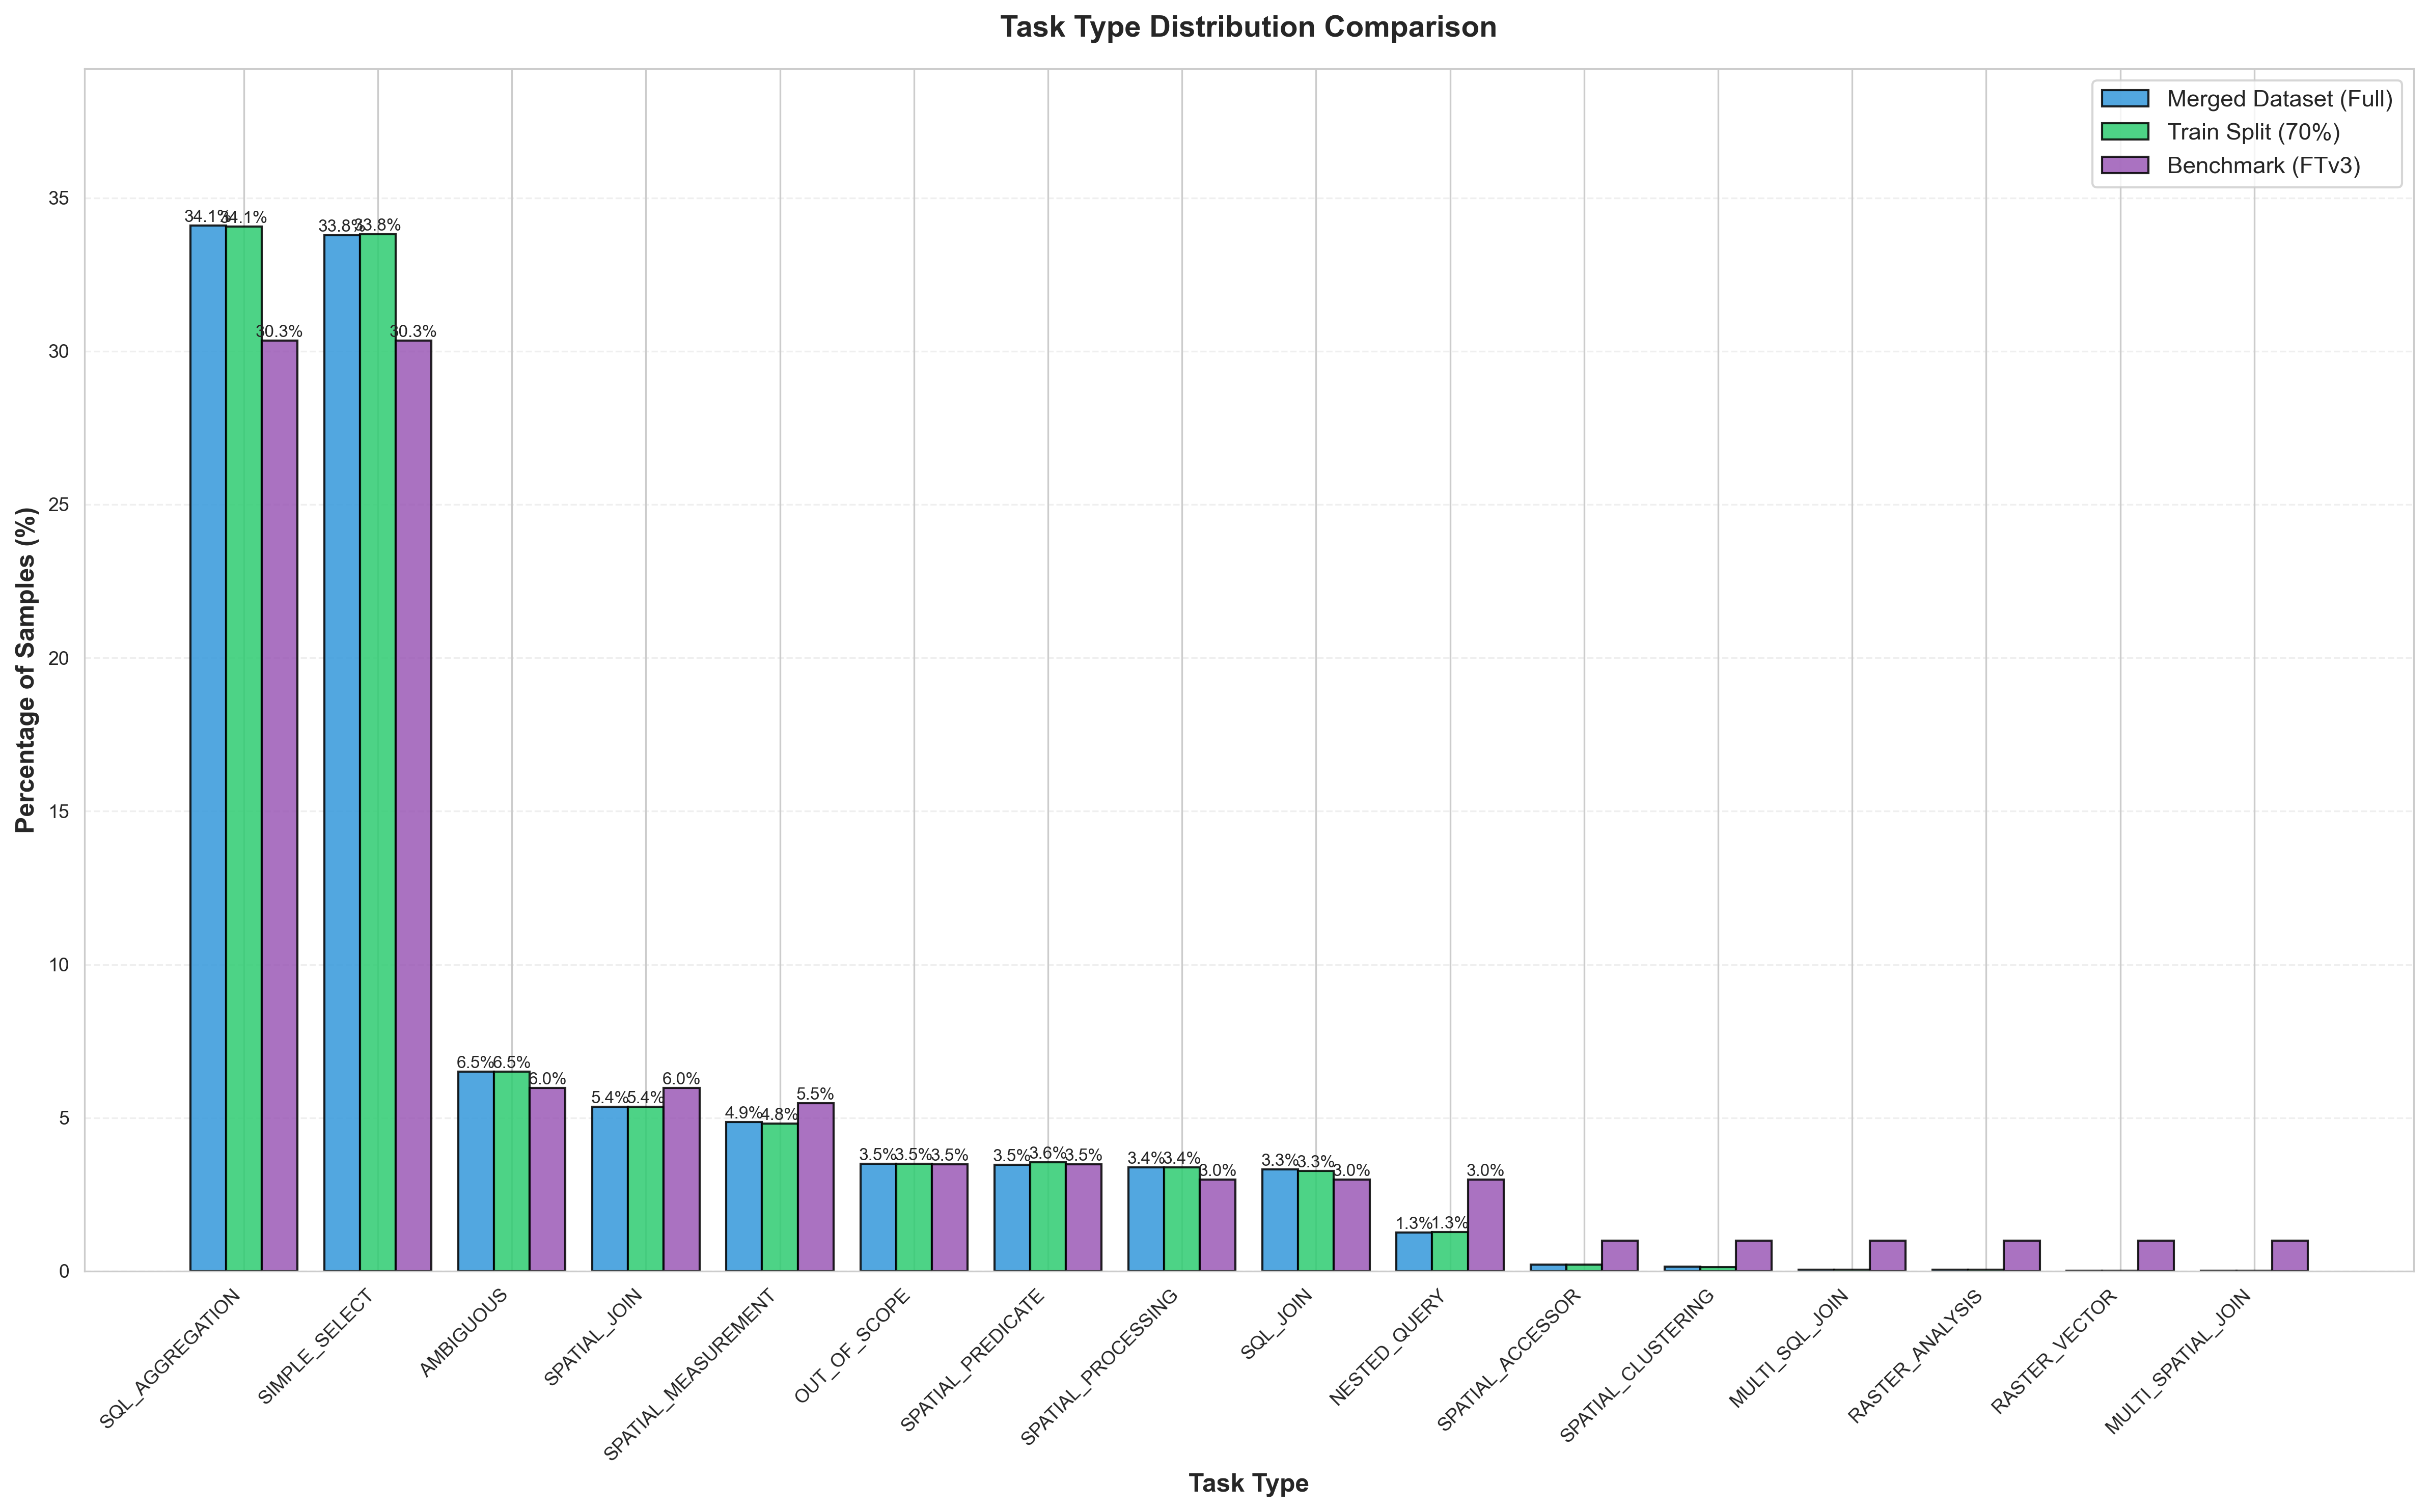
\includegraphics[width=0.95\textwidth]{Figures/02_task_type_comparison.png}
\caption{Task type distribution: Merged dataset vs Training set. Stratification preserves frequency-based distribution across all dimensions.}
\label{fig:stratification}
\end{figure}

\section{Benchmark and Model Evaluation}

The evaluation benchmark contains 201 stratified samples with 100\% executable ground truth. Fine-tuned SQLCoder 7B achieves \textbf{84.58\% execution accuracy (EX)}, outperforming GPT-4o (30.85\%) by \textbf{54 percentage points} despite being 14x smaller. The radar chart (Figure~\ref{fig:radar}) reveals that SQLCoder demonstrates consistent performance across all metrics (Deep EM: 81.59\%, SC: 63.18\%), while frontier models achieve high structural correctness but lack PostGIS domain knowledge. By task type: SIMPLE\_SELECT achieves 96.72\%, SPATIAL\_JOIN 88.89\%, and SPATIAL\_PREDICATE 100\%. Self-correction shows minimal improvement (EA = EX = 84.58\%), with 89\% first-shot success, validating that quality training data outweighs iterative refinement.

\begin{figure}[H]
\centering
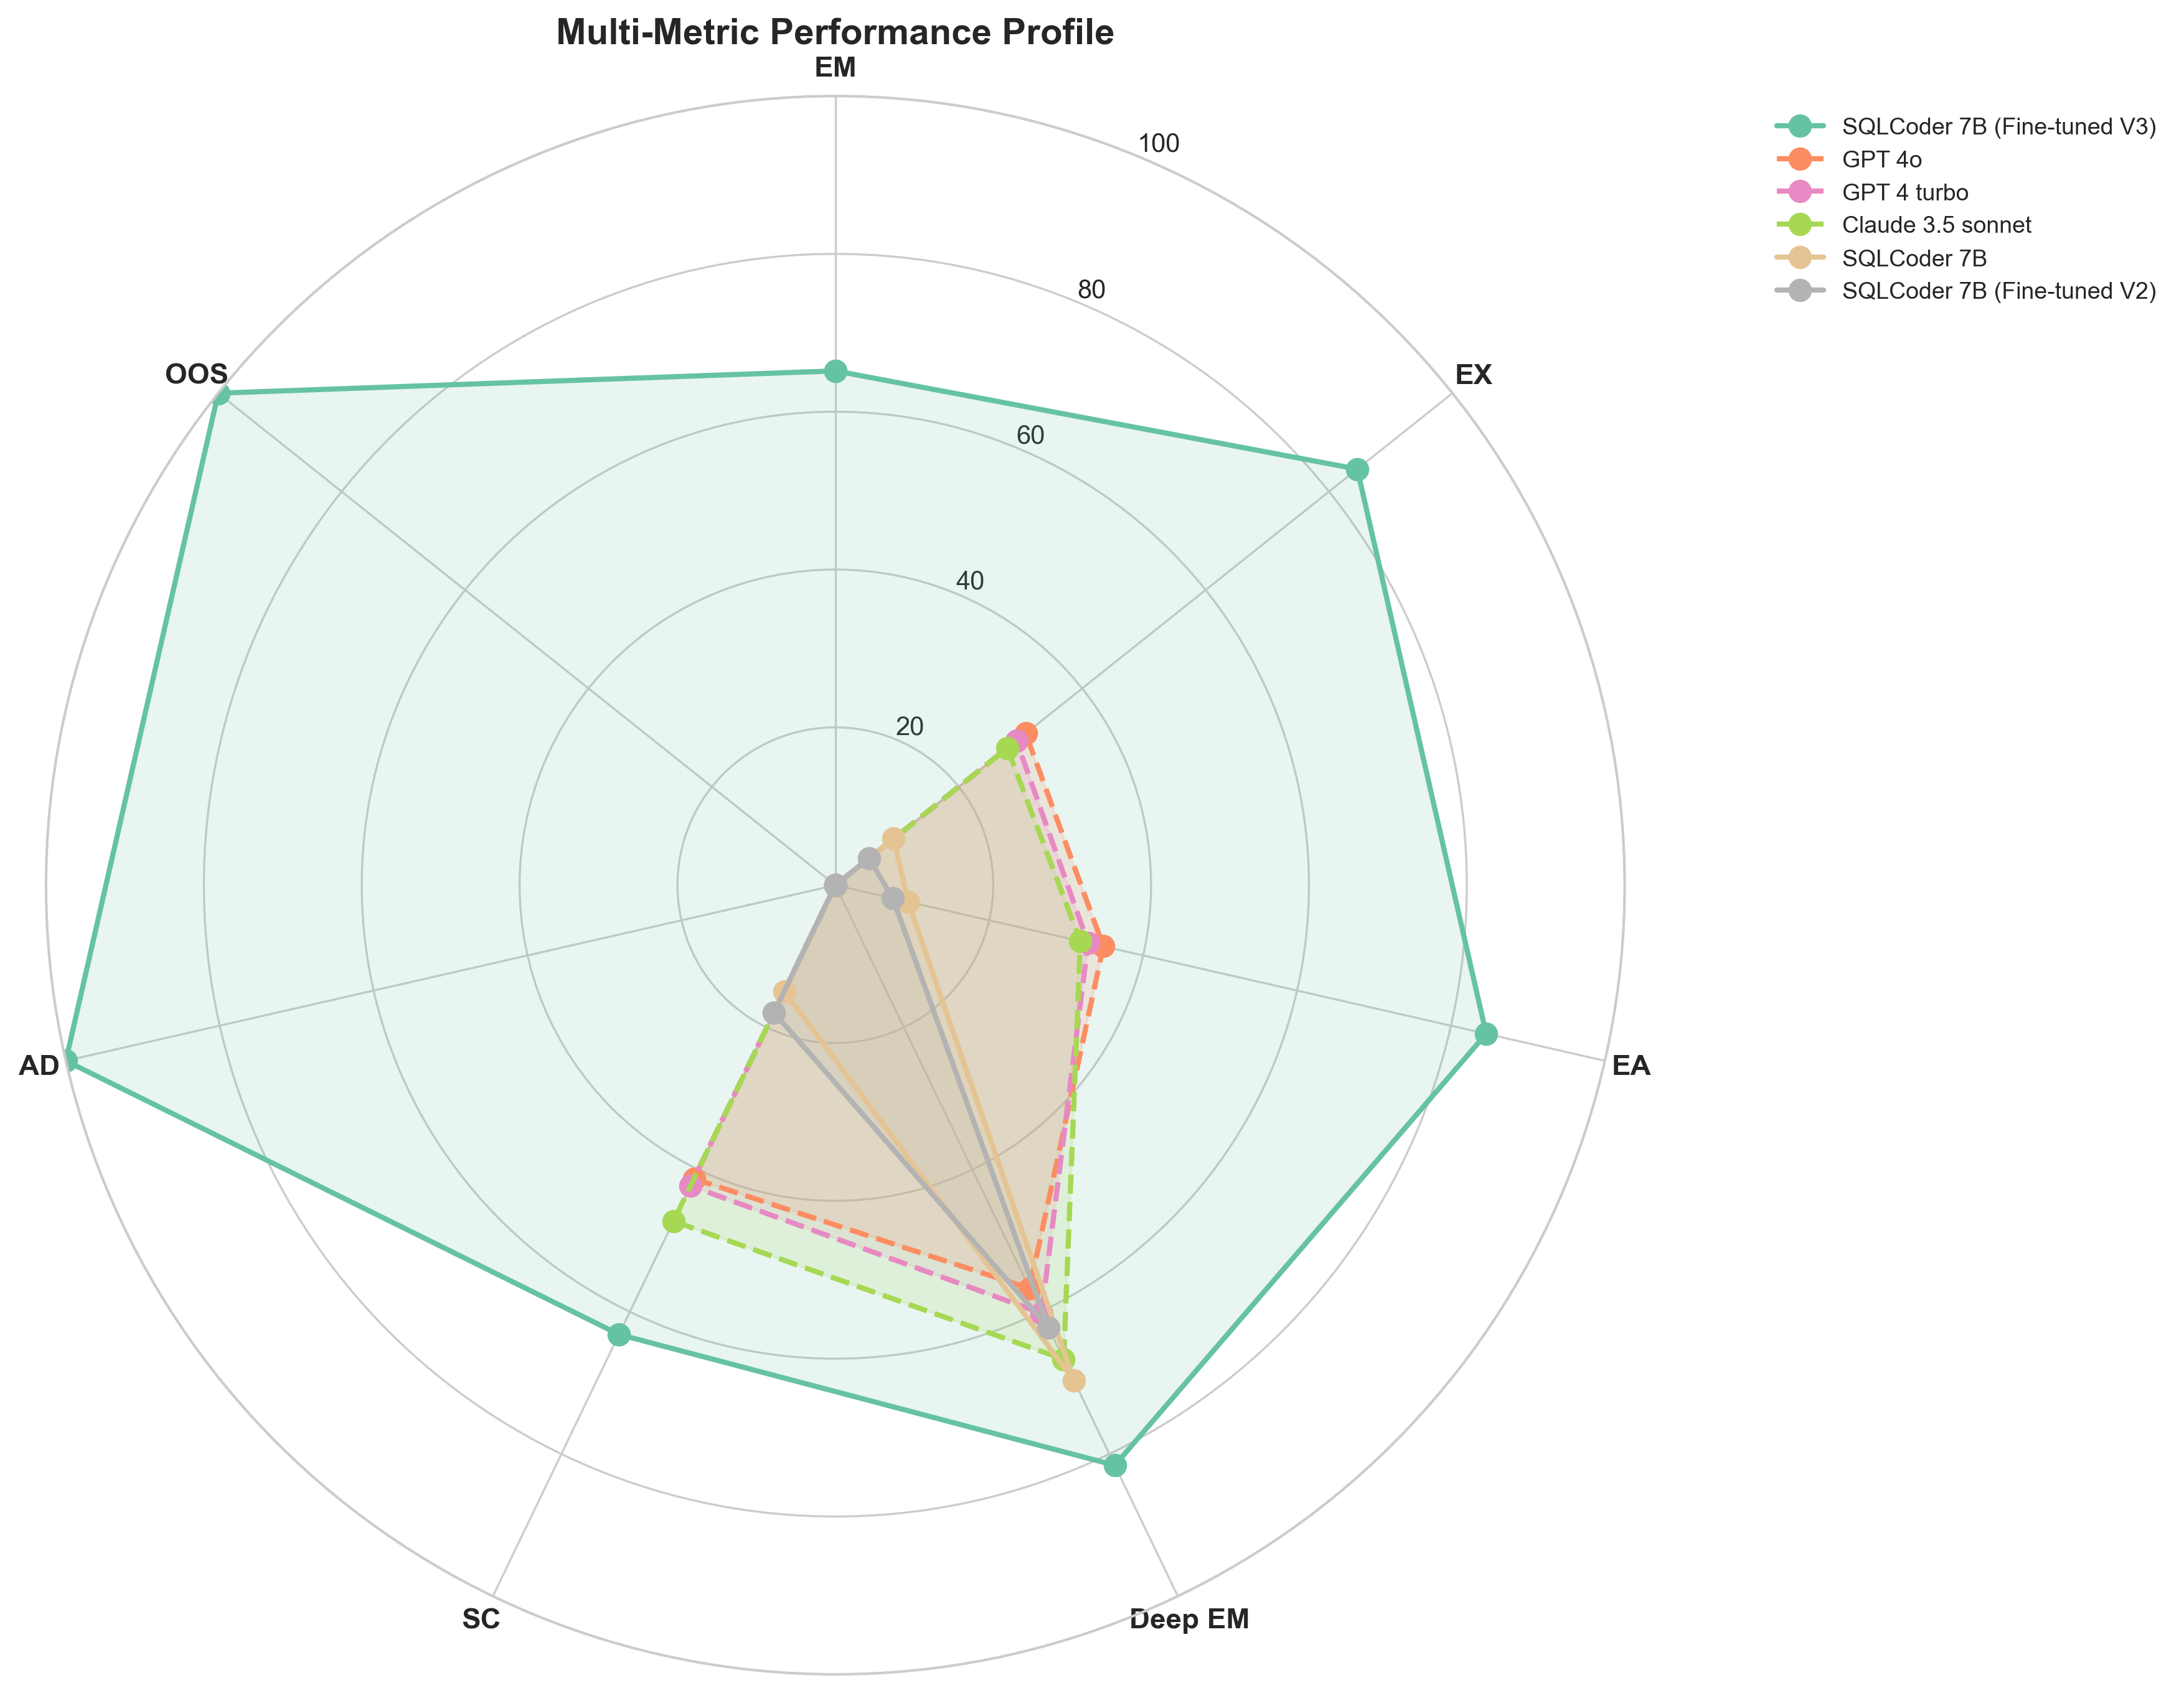
\includegraphics[width=0.95\textwidth]{Figures/performance/radar_comparison.png}
\caption{Radar chart: Model capabilities across execution accuracy, structural correctness, and semantic validity.}
\label{fig:radar}
\end{figure}

\section{Fine-Tuning and Efficiency}

SQLCoder 7B was fine-tuned using QLoRA on an RTX 6000 24GB GPU at Politecnico di Torino's IPAZIA cluster. Training completed in 51 hours (2,187 steps), achieving final loss of 0.036 with 18GB memory usage (75\% utilization). The model demonstrated 51\% faster training and 25\% better convergence than larger alternatives, with academic GPU access providing \$33-88 savings versus commercial platforms.

\section{Key Achievements}

\begin{itemize}
\item \textbf{Dataset}: 50,000 samples at \$50 with 97.34\% NoErr (3,600x cost reduction)
\item \textbf{Performance}: 84.58\% EX, outperforming frontier models by 54 points
\item \textbf{Production-ready}: 1.2s inference, 89\% first-shot success, 91.2\% out-of-scope detection
\item \textbf{Open-source}: CIM Wizard (13,522 LOC), dataset on HuggingFace (\texttt{taherdoust/ai4cimdb})
\end{itemize}

This work establishes SQLCoder 7B with QLoRA as the recommended approach for PostGIS Text-to-SQL, demonstrating that domain-specific fine-tuning on curated datasets achieves production-ready performance at minimal cost, with methodology applicable beyond urban energy modeling.

\end{document}
